\chapter{Interfaces and Validation}
\section{Interface Overview}
Signed-in users can open the anomaly, risk, login-log, and AI investigation pages. Administrators also have navigation to the global dashboard, directory, and audit records. The backend decides whether a request is authorized, regardless of which links the frontend displays.

Login and registration sit outside the protected layout. The authentication context keeps the token and safe user details in local storage. The shared HTTP client attaches the bearer token and clears the session on relevant unauthorized responses. Directory controls change account state. The audit view displays security records, while the browser console provides diagnostics.

Users can filter anomalies by rule type and severity and inspect their event context. The risk page summarizes the preceding 24 hours. Login views show the records behind the alerts, including administrator-created demonstration events. In the AI workspace, users select investigator, operator, or collaborative behavior and submit a prompt with optional context, steering, and follow-up arrays. The returned trace shows tool outcomes.

\clearpage\section{Application Screenshots}
These six candidate-provided captures show sign-in, overall monitoring, event investigation, personal risk, and the AI workspace. Their displayed content is unchanged. Counts and scores belong to the captured demonstration state; they are not evaluation measurements.

\begin{figure}[!ht]\centering
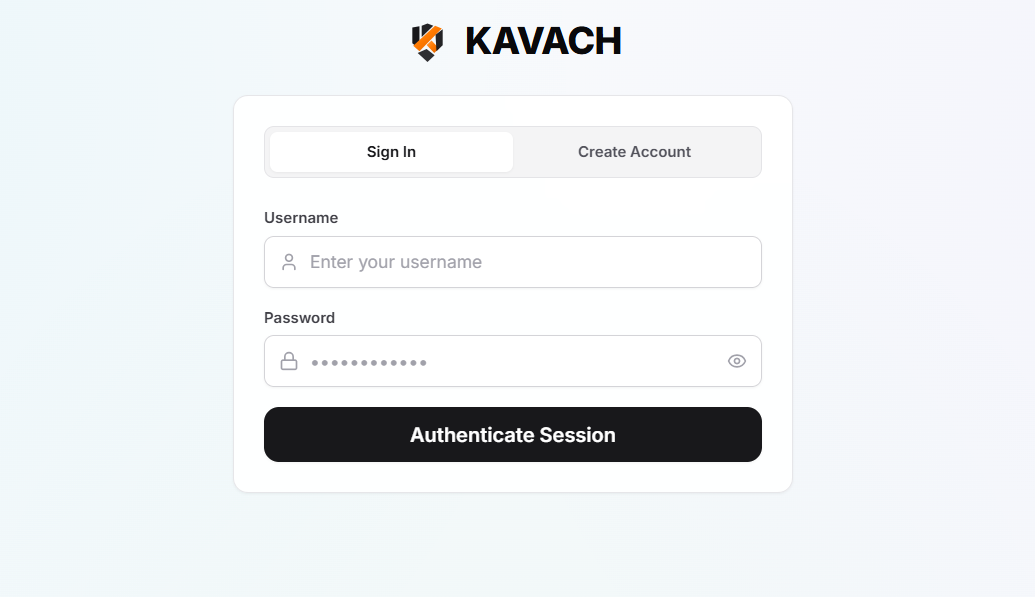
\includegraphics[width=.75\textwidth]{images/screenshot-login.png}
\caption{Sign-in interface with account-registration tab and authentication form.}\label{fig:screen-login}
\end{figure}

\begin{figure}[!ht]\centering
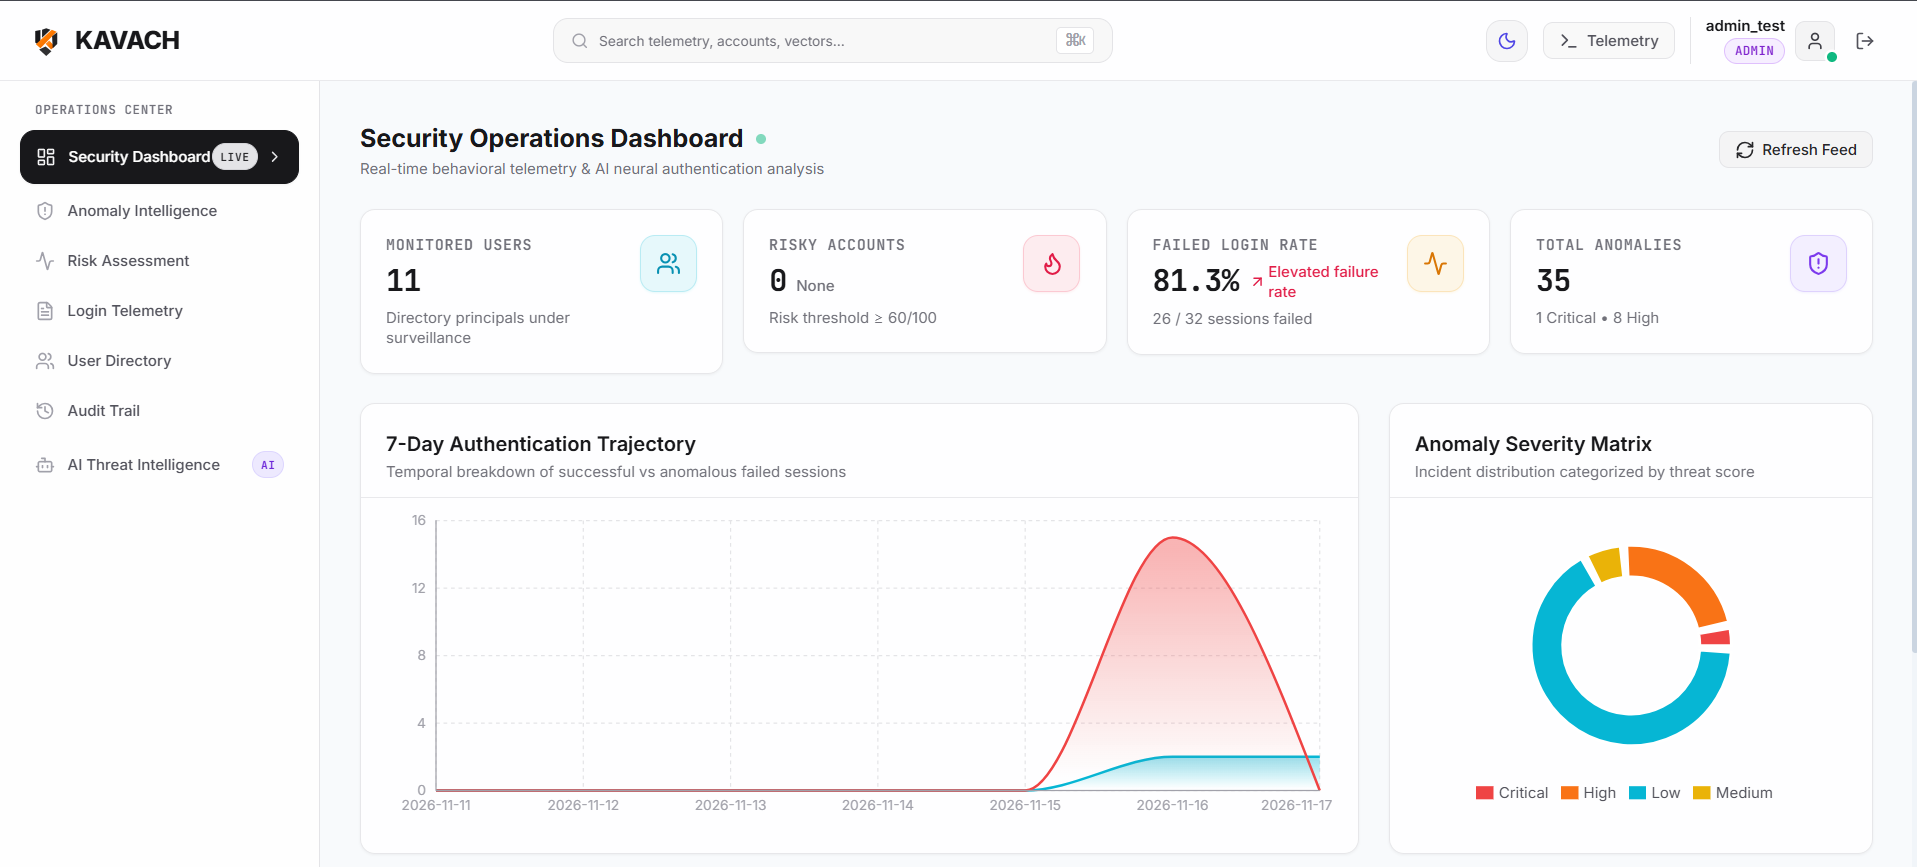
\includegraphics[width=\textwidth]{images/screenshot-dashboard.png}
\caption{Administrator dashboard: account counts, login outcomes, trend, and anomaly severity.}\label{fig:screen-dashboard}
\end{figure}

\clearpage\subsection{Anomaly Investigation and Login Telemetry}
The anomaly list shows matching rules and their alert weights. The login view provides the underlying event fields. Filters and action buttons are visible, but the captures do not show what happened after those actions were selected.

\begin{figure}[!ht]\centering
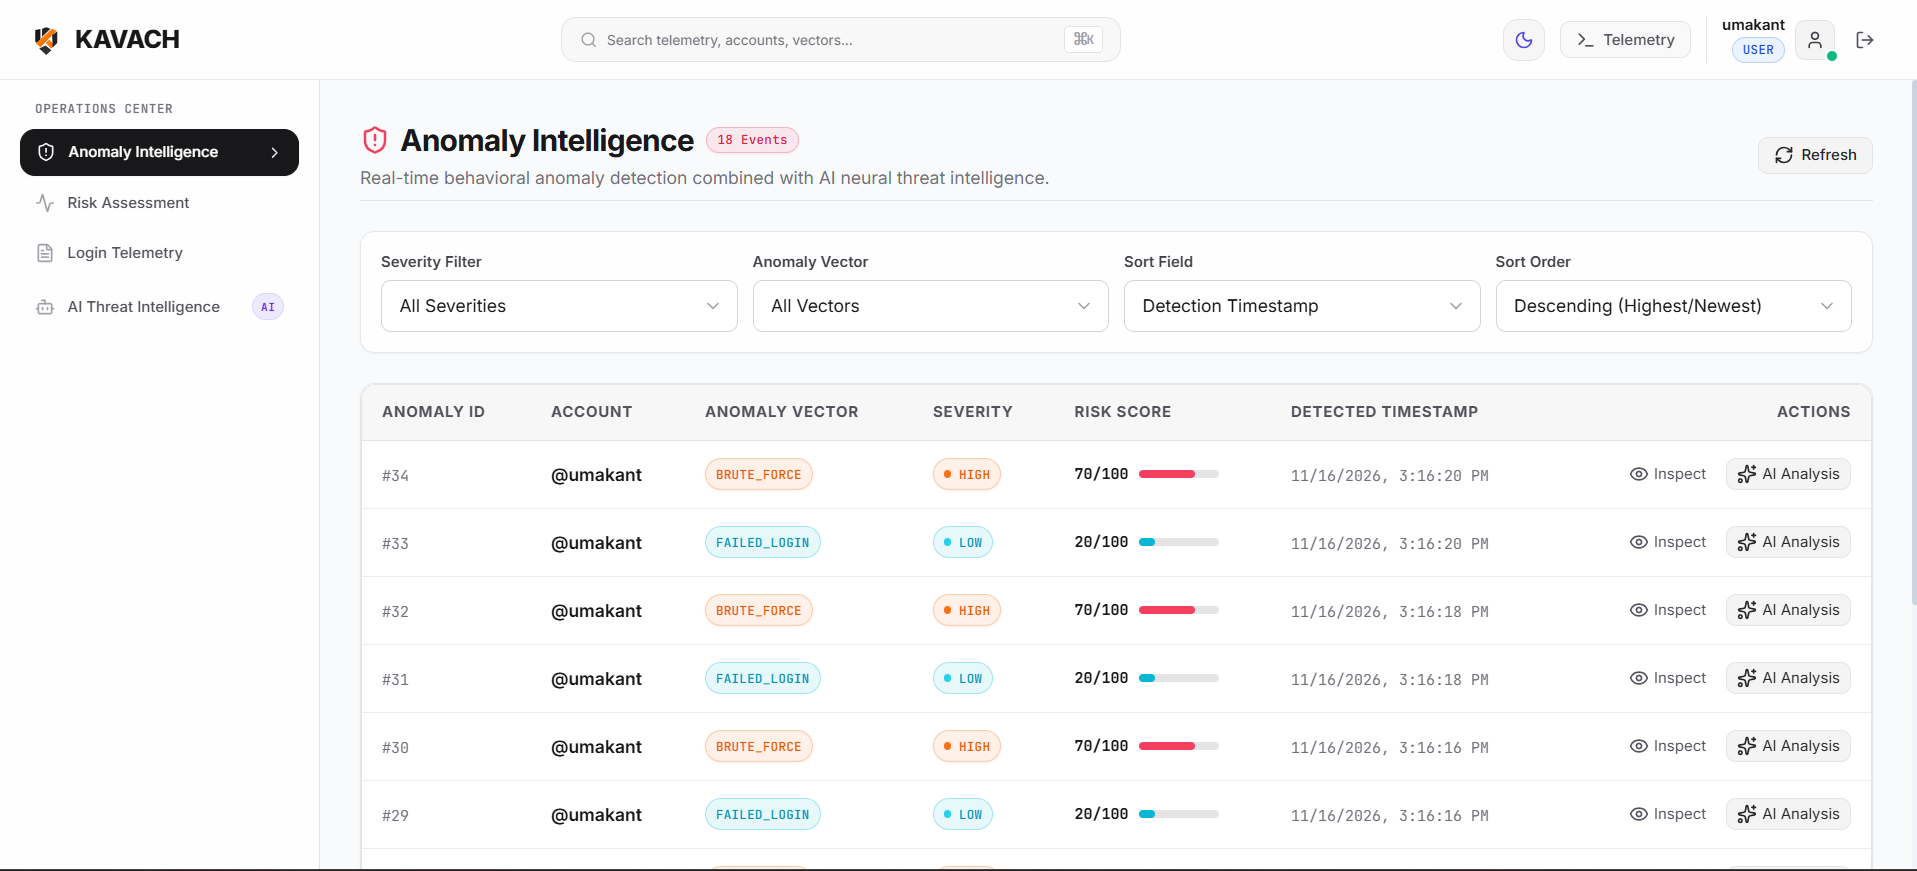
\includegraphics[width=\textwidth]{images/screenshot-anomalies.png}
\caption{User-scoped anomaly list with filters, rule types, severity, and alert weights.}\label{fig:screen-anomalies}
\end{figure}

\begin{figure}[!ht]\centering
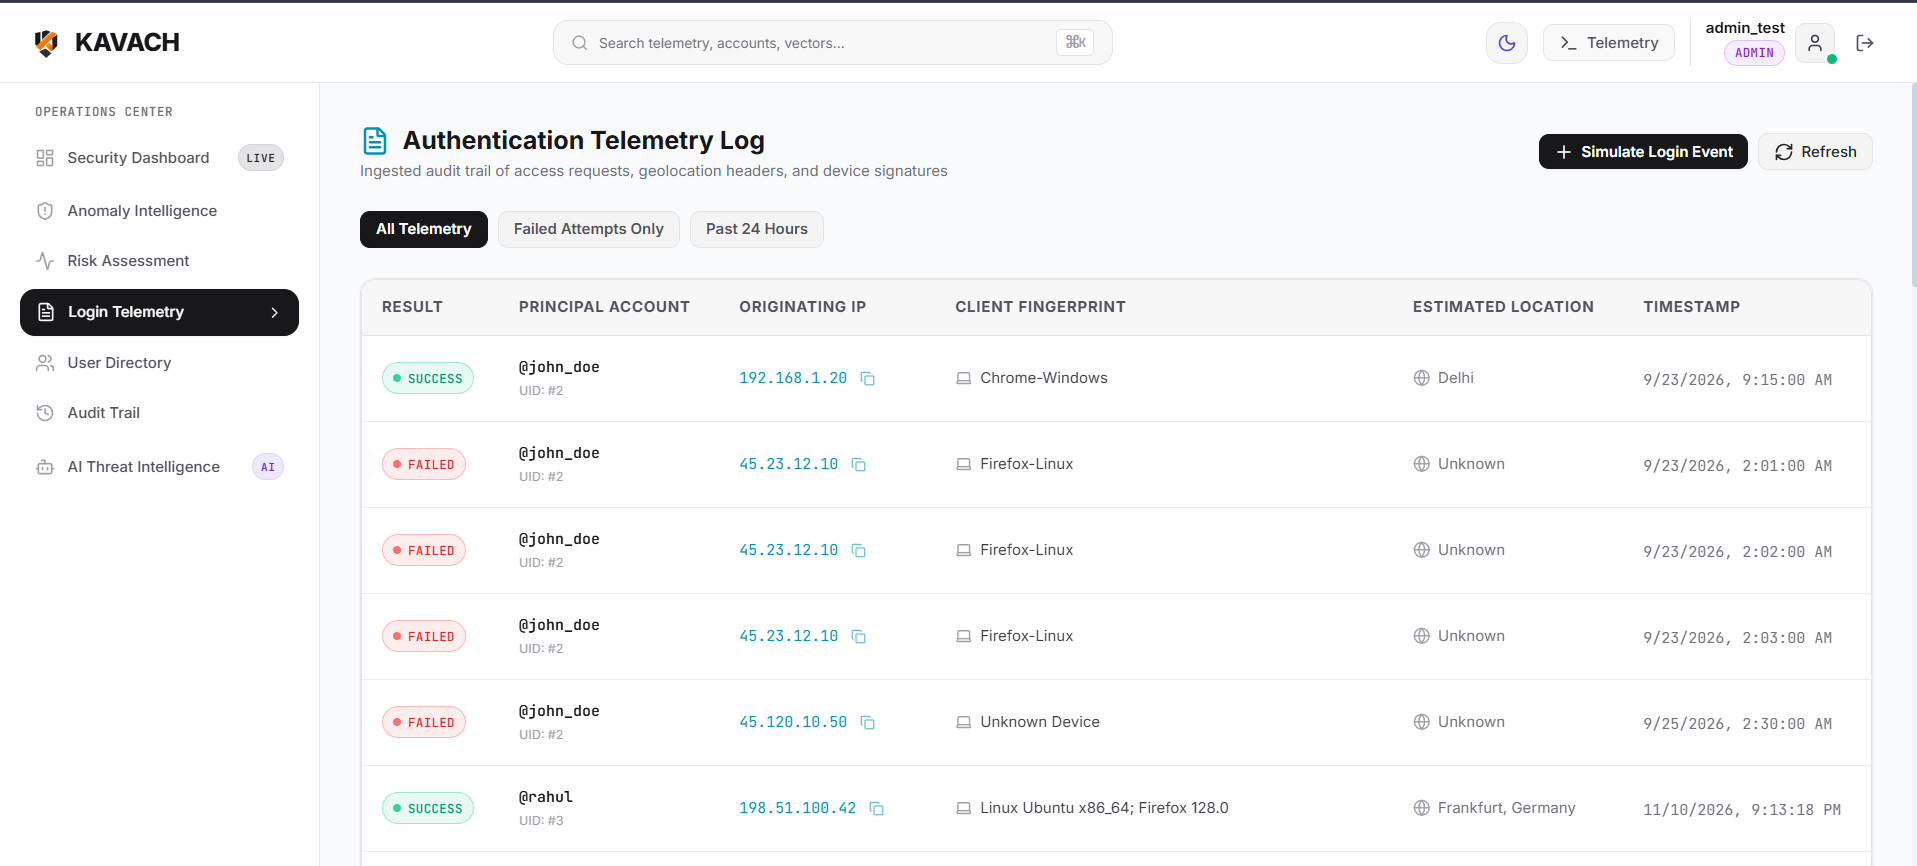
\includegraphics[width=\textwidth]{images/screenshot-telemetry.png}
\caption{Login telemetry showing successful and failed events with account and client metadata.}\label{fig:screen-telemetry}
\end{figure}

\clearpage\subsection{Personal Risk and AI Workspace}
The personal page shows the signed-in account's risk profile. Its recent 24-hour score and historical anomaly counts cover different periods. Although the interface uses subtitles such as ``Bayesian'' and ``neural'', Chapter 4 describes the implemented fixed rules and additive score. The AI screenshot captures the initial console before any completed model or tool execution.

\begin{figure}[!ht]\centering
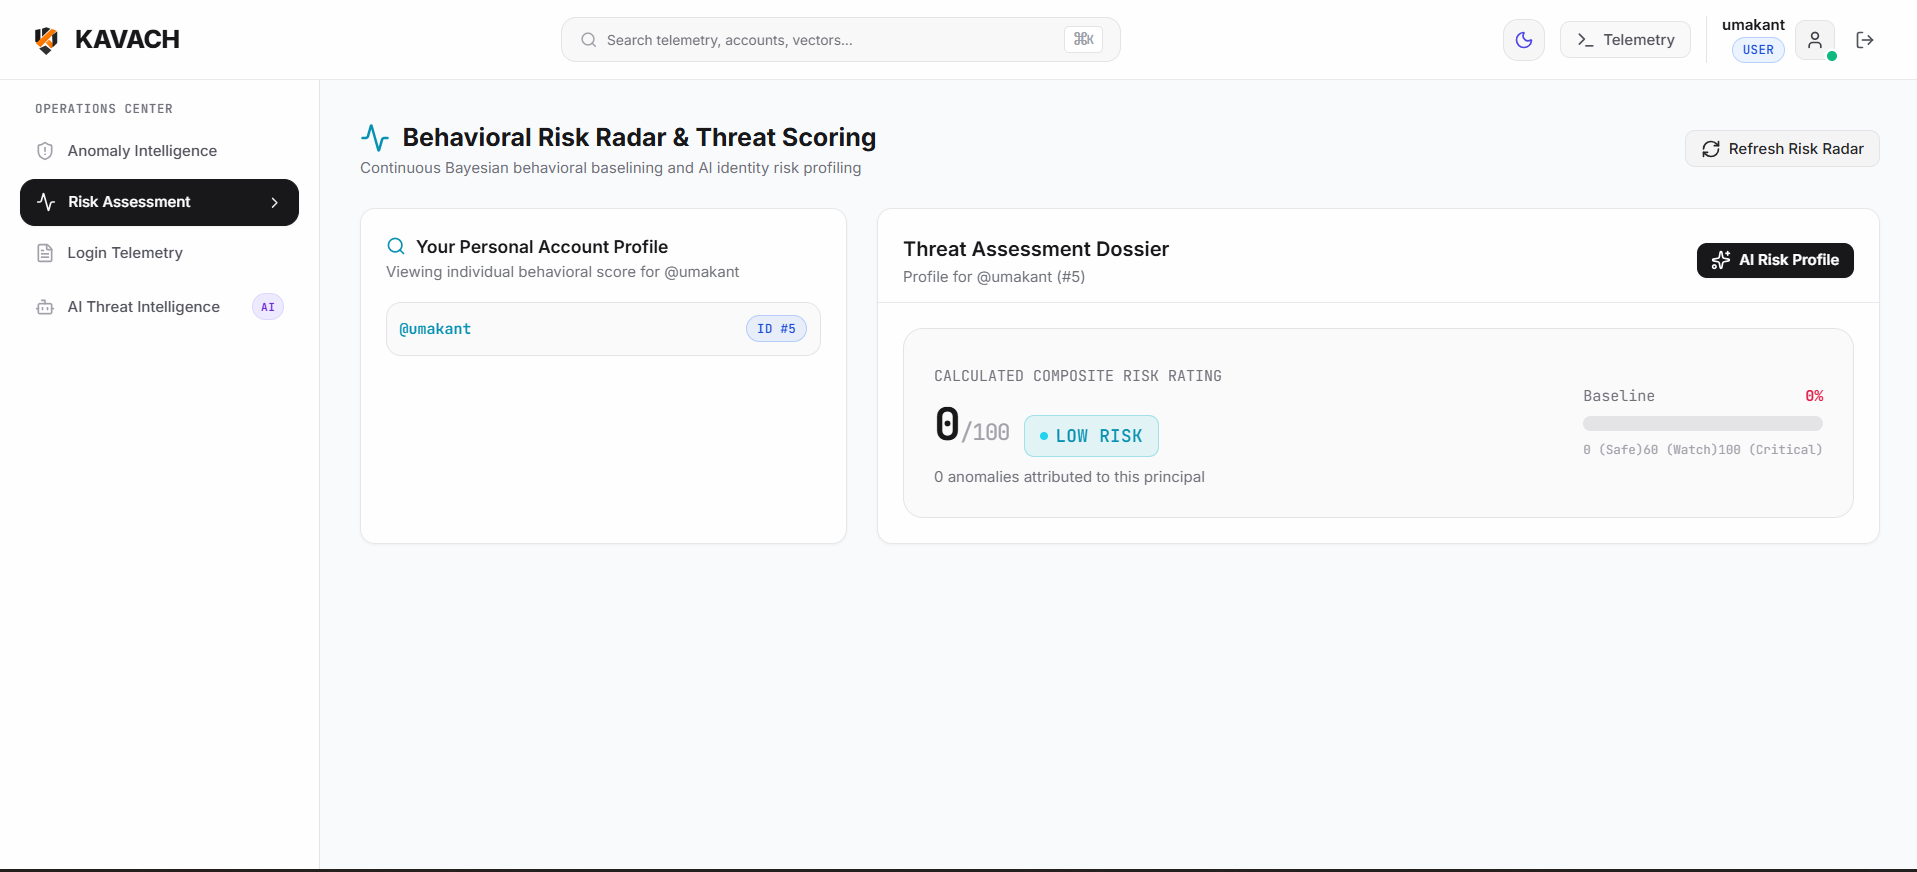
\includegraphics[width=\textwidth]{images/screenshot-personal-risk.png}
\caption{Personal risk view for the USER account, showing the displayed score and profile.}\label{fig:screen-risk}
\end{figure}

\begin{figure}[!ht]\centering
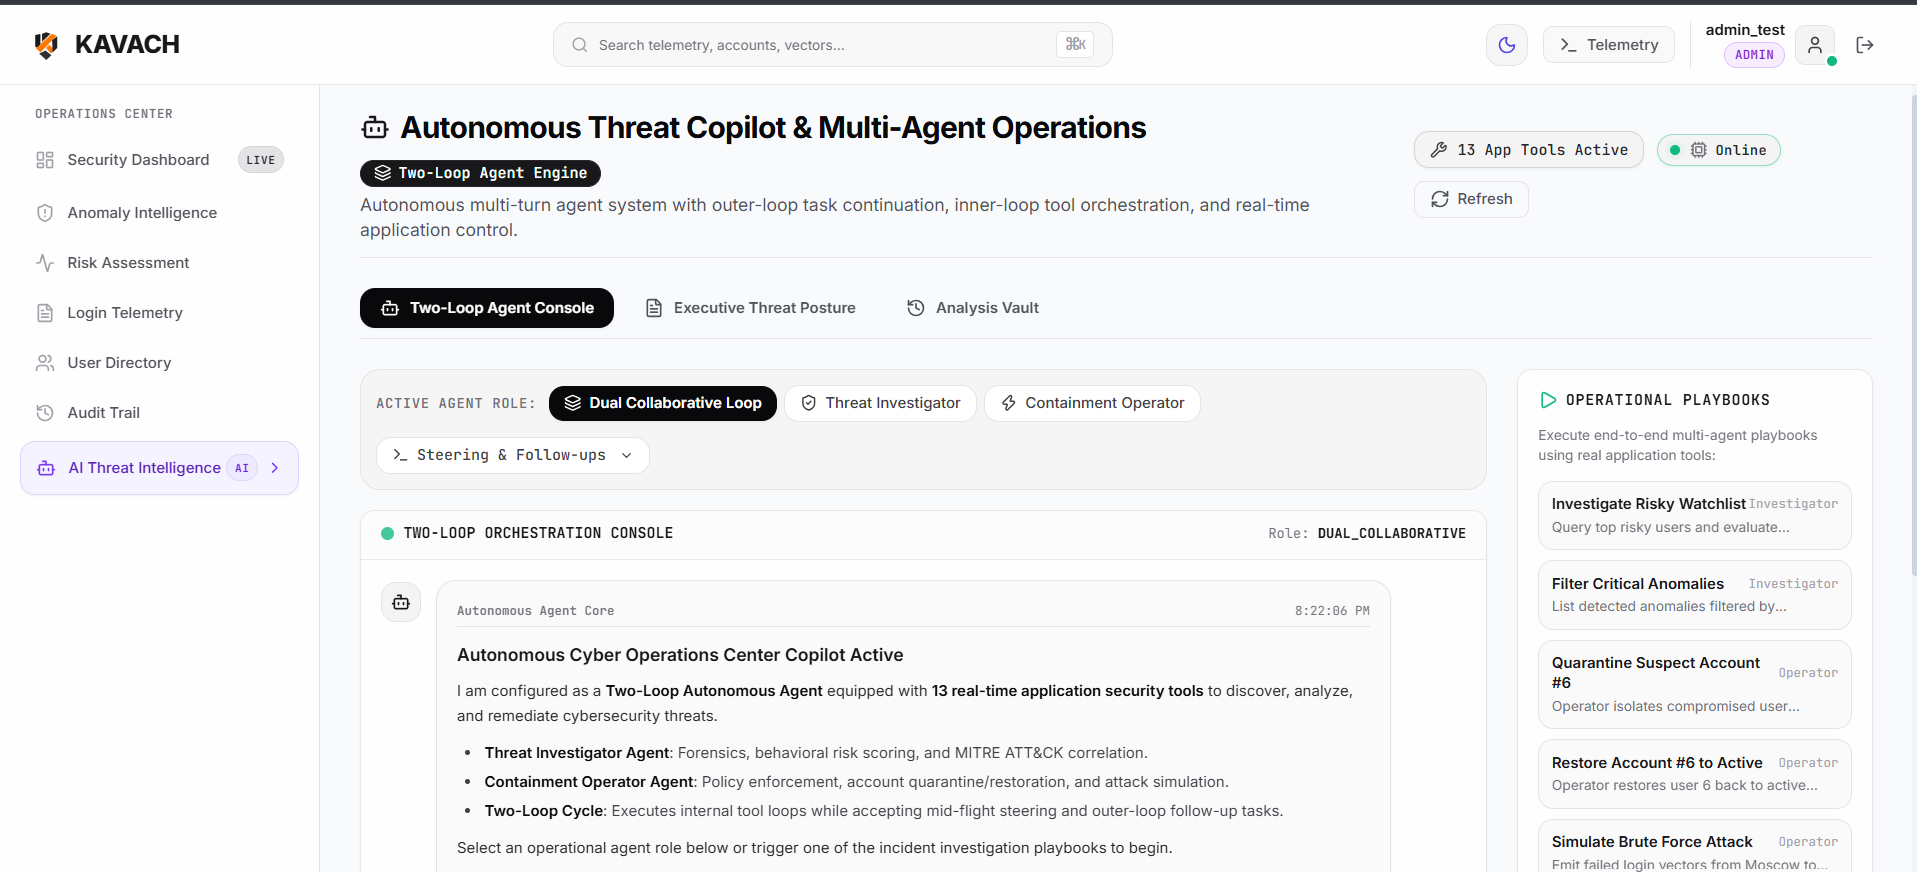
\includegraphics[width=\textwidth]{images/screenshot-ai-console.png}
\caption{AI workspace with agent-role selection, a 13-tool indicator, and operational playbooks.}\label{fig:screen-ai}
\end{figure}


\clearpage\section{Validation Plan}
The screenshots show interface states captured by the candidate. The repository has a context-loading test, but the project materials contain no controlled rule-test or load-test results. Table~\ref{tab:tests} defines the inputs and expected outcomes for validation; none of these rows records a test pass.
\begingroup\footnotesize\setstretch{1.0}\renewcommand{\arraystretch}{1.1}\setlength{\parskip}{0pt}
\begin{longtable}{>{\raggedright\arraybackslash}p{0.9cm}>{\raggedright\arraybackslash}p{6.1cm}>{\raggedright\arraybackslash}p{7cm}}
\caption{Functional validation plan; execution pending.}\label{tab:tests}\\\toprule ID & Input / action & Expected behavior to verify\\\midrule\endfirsthead
\toprule ID & Input / action & Expected behavior to verify\\\midrule\endhead
T1 & Register unique credentials. & Active USER, encoded password, safe response, audit event.\\
T2 & Repeat username or email. & Conflict and no duplicate account.\\
T3 & Valid password for active user. & JWT, success telemetry, applicable contextual rules.\\
T4 & Incorrect password for known user. & Unauthorized; failed telemetry and failed-login anomaly.\\
T5 & Unknown username. & Audit failure; no user-linked login record.\\
T6 & Inactive account attempts login. & Forbidden; failed telemetry and inactive-user anomaly.\\
T7 & Events at 04:59 and 05:00. & Unusual-time alert only before 05:00.\\
T8 & First event, repeated values, unseen IP/device. & No initial new-value alerts; later unseen values trigger.\\
T9 & Four then five failures in window. & Fifth qualifying failure adds brute-force anomaly.\\
T10 & Reanalyse identical login event. & No duplicate event/user/rule anomaly in sequential execution.\\
T11 & Weight totals 29, 30, 59, 60, 79, 80, 120. & Correct boundary tiers; score capped at 100.\\
T12 & Move anomaly detection time beyond 24 hours. & Expired anomaly excluded from risk.\\
T13 & Deactivate account with issued JWT. & Subsequent protected request rejected.\\
T14 & Make live inference unavailable. & Deterministic fallback with accurate status and outcomes.\\
T15 & Submit steering and two follow-ups. & Inner context consumes steering; outer cycles consume follow-ups.\\\bottomrule
\end{longtable}
\endgroup

Further tests must check cross-account access and administrative actions through both endpoints and tools. They must also cover invalid arguments, malformed model output, provider failures, concurrent inserts, and backdated events.

Detection evaluation requires labelled ordinary and suspicious events, with precision and recall measured for each rule. Performance results must record hardware, data volume, concurrency, latency, and whether inference was live or in fallback mode. Deterministic and model-assisted results need separate measurements.
